\documentclass[tikz,border=5pt]{standalone}
\usepackage{amsmath,amssymb}
\usetikzlibrary{arrows.meta,positioning}
\definecolor{curveblue}{HTML}{245C86}
\definecolor{accent}{HTML}{A65E2E}
\begin{document}
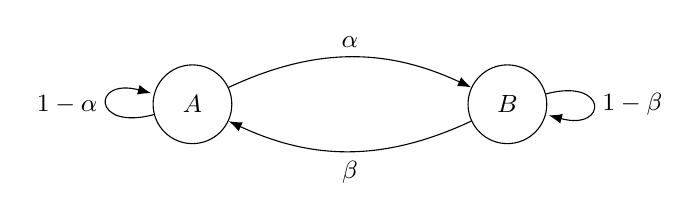
\begin{tikzpicture}[font=\small,>=Latex,line cap=round,line join=round]

\node[draw,circle,minimum size=10mm] (a) at (0,0) {$A$};
\node[draw,circle,minimum size=10mm] (b) at (4,0) {$B$};
\draw[->] (a) to[bend left=25] node[above]{$\alpha$} (b);
\draw[->] (b) to[bend left=25] node[below]{$\beta$} (a);
\draw[->] (a) edge[loop left] node[left]{$1-\alpha$} (a);
\draw[->] (b) edge[loop right] node[right]{$1-\beta$} (b);
\end{tikzpicture}
\end{document}
